%========================================================================================
% TU Dortmund, Informatik Lehrstuhl VII
%========================================================================================

\chapter{Graphische Ausgabe}
\label{Kapitel 2}
%
(Hier kurze Einleitung und Bild der Spielszene)


\section{Rendering Architektur}
\label{Kapitel_2_-_Unterkapitel_1}
%
(Hier Bild des Rendering-Systems und kurze Erklärungen zu den einzelnen Renderables)
\begin{figure}[h]
	\centering
	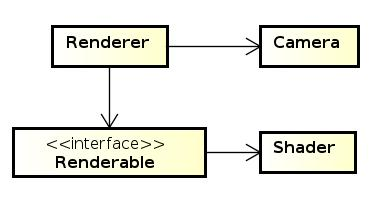
\includegraphics[width=0.6\linewidth]{bilder/RenderingSystem}
	\caption{Klassen des Rendering-Systems}
\label{fig:renderingSystem}
\end{figure}

\section{Partikelsystem}
\label{Kapitel_2_-_Unterkapitel_2}
%
Partikelsysteme sind in interaktiven Anwendungen wie Computerspiele und in der Postproduktion von Filmen, seien es Real- oder Animationsfilme, allgegenwärtig.
Man denke an typische Effekte wie Feuer und Rauch, aber auch Flüssigkeiten lassen sich mithilfe von Partikelsystemen realisieren.

Nach \cite{reeves:particle_systems} sind Partikelsysteme besonders geeignet für Objekte die sich aufgrund ihrer Komplexität nur schwer mit einem Mesh darstellen lassen und sich im Verlauf der Zeit in ihrer Form ändern. Eine einfache Repräsentation solcher Objekte lässt sich daher mit Wolken aus Partikeln umsetzen, wobei die Partikel einfache Primitive wie Punkte, Linien und Dreiecke sind\cite{reeves:particle_systems}.

In der Anwendung wird ein Partikelsystem genutzt um den Flugverlauf des Balles darzustellen. Dabei sind die Partikel Quads, bestehend aus jeweils 6 Vertices, auf die eine Textur projiziert wird.

\subsection{Komponenenten des Partikelsystems}
\label{Kapitel_2_-_Unterkapitel_2.1}
%
In der Anwendung besteht das Partikelsystem aus zwei Klassen, nämlich dem {\texttt{Particle}} und dem {\texttt{BallParticleRenderable}}.

Die {\texttt{Particle}} Klasse repräsentiert ein Partikel, welches eine Position in Weltkoordinaten, eine Geschwindigkeit, eine Lebensdauer und eine Größe hat. 
Die {\texttt{BallParticleRenderable}} Klasse ist für die Darstellung und Verwaltung aller im System vorhandenen Partikel zuständig. Zur Verwaltung gehört das emittieren neuer Partikel, das Aktualisieren der aktiven Partikel und Löschen der ‚toten‘ Partikel, also solcher, deren Lebensdauer null erreicht hat. Die Klasse hält Attribute, die die maximale Anzahl der aktiven Partikel beschränkt sowie die Emittiergeschwindigkeit.  Sie hat auch ein Attribut für die Position. Alle neuen Partikel werden relativ zu dieser Position emittiert. Dabei ist die Position des Emittierpunktes auf dem Rand des Balles entgegengesetzt dem Geschwindigkeitsvektor des Balles.

\subsection{Instanced Rendering}
\label{Kapitel_2_-_Unterkapitel_2.2}
%
Instanced Rendering bezeichnet eine effiziente Variante des Renderns von Objekten die dieselben Renderdaten verwenden, sich aber nur darin unterscheiden, wo sie im Weltkoordinatensystem platziert werden. Für die Partikel unseres Partikelsystems trifft dies zu, da jedes Partikel, wie bereits erwähnt, ein einfaches Quad ist und sich nur in seiner Position und Größe unterscheidet.

Die Effizienz dieser Methode rührt daher, dass zum Rendern der Partikel nun nicht mehr über die Liste aller Partikel iteriert wird und für jedes Partikel ein Draw-Call getätigt wird. Stattdessen wird pro Frame nur ein einziger Draw-Call getätigt, das heißt, dass nur ein Befehl über den langsamen Peripheriebus zur Grafikkarte gesendet werden muss. Für das Instanced Rendering bietet OpenGL die Funktionen {\texttt{glDrawArraysInstanced}} und {\texttt{glDrawElementsInstanced}}.

Um nicht zu sehr in den technischen Details zu versinken, soll nur kurz schematisch anhand von Abbildung \ref{fig:vao} der Vorgang beim Rendern der Partikel erläutert werden.
%Todo vao bild;kurz auf performance eingehen; verweis auf super bible

\begin{figure}[h]
	\centering
	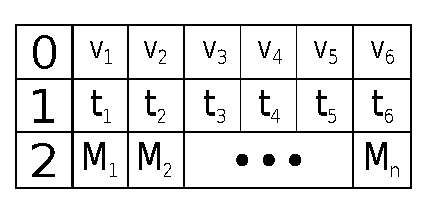
\includegraphics[scale=0.8]{bilder/vao}
	\caption{VAO im {\texttt{BallParticleRenderable}} nach jedem Update der Partikel}
	\label{fig:vao}
\end{figure}

Wie an Abbildung \ref{fig:vao} zu sehen ist, befinden sich die Vertizes $v_1\dotsc v_6$ , die Texturkoordinaten $t_1\dotsc t_6$ und die Model-Matrizen $M_1\dotsc M_n$, wobei $\mathnormal{n}$ die Anzahl der aktiven Partikel ist, in ihren eigenen Array-Buffer. Die Vertices und Texturkoordinaten ändern sich nicht. Die Model-Matrizen hingegen werden bei jedem Update der Partikel neu erzeugt und an den Array-Buffer gesendet.

Um Instanced Rendering zu nutzen muss der Array-Buffer der Model-Matrizen als Instance-Attribut des Vertex-Shaders deklariert werden. Dies sollte bei der Assoziation der Array-Buffer mit den Attributen des Vertex-Shader-Programms geschehen.
Beim Rendern einer Instanz werden nun alle Vertexdaten und Texturkoordinaten, die keine Instanz-Variablen sind, und die jeweilige Model-Matrix der Instanz verwendet.

Für weitere Informationen zum Thema Instanced Rendering sei auf \cite{ksls:2013} verwiesen.

\subsection{Blending und Tiefentest}
\label{Kapitel_2_-_Unterkapitel_2.3}
%
In dem verwendeten Partikelsystem sollen die Farben der Partikel, wenn sie sich überlagern, addiert werden. Der resultierende Effekt ist, dass bei genügend sich überlagernden Partikel ein leuchtend weißer Bereich zu sehen ist. Blending erlaubt es, Farben miteinander zu vermischen und ist ein Teil der Verarbeitung der Fragmente in der Rendering Pipeline. OpenGL bietet verschiedene Blending-Arten an, die durch den Aufruf der Funktion {\texttt{glBlendFunc}} eingestellt werden können. 

\begin{figure}[h]
\centering
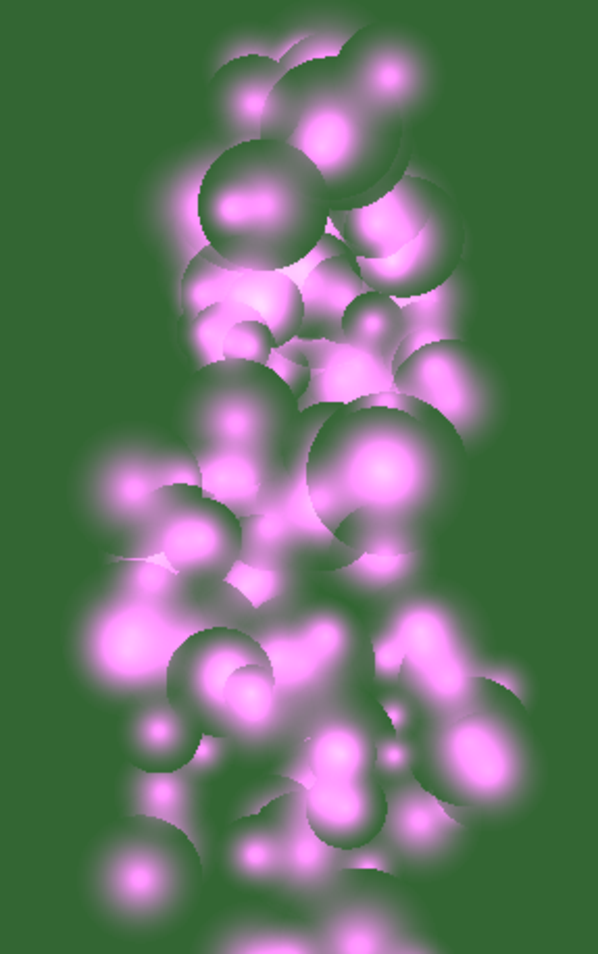
\includegraphics[scale=0.4]{bilder/BlendingEnabled}
\caption{Partikelsystem bei aktiviertem Blending}
\label{fig:BlendingEnabled}
\end{figure}

Abbildung \ref{fig:BlendingEnabled} zeigt wie das Partikelsystem bei eingeschaltetem Blending und Verwendung von {\texttt{glBlendFunc}} mit den Argumenten {\texttt{GL\_SRC\_ALPHA}} und {\texttt{GL\_ONE}} aussieht. Eine Übersicht über die verschiedenen Argumente für {\texttt{glBlendFunc}} und ihre Auswirkungen auf die Farbe eines Fragments ist in \cite{virag:2012} zu finden.

Wie an Abbildung \ref{fig:BlendingEnabled} zu erkennen ist tritt trotz eingeschaltetem Blending der gewünschte Effekt nicht auf. Grund dafür ist der Tiefentest. Für den Tiefentest spielt es keine Rolle, ob ein Fragment teilweise transparent ist, da der Tiefenwert für ein Fragment trotzdem in den Tiefenpuffer geschrieben wird, vorausgesetzt der Wert ist geringer.

Um dies zu umgehen, lässt sich mittels der Funktion {\texttt{glDepthMask}} das Schreiben in den Tiefenpuffer für das Rendern der Partikel verbieten.
Das endgültige Resultat ist in Abbildung \ref{fig:ParticleFinal} zu sehen.

\begin{figure}[h]
	\centering
	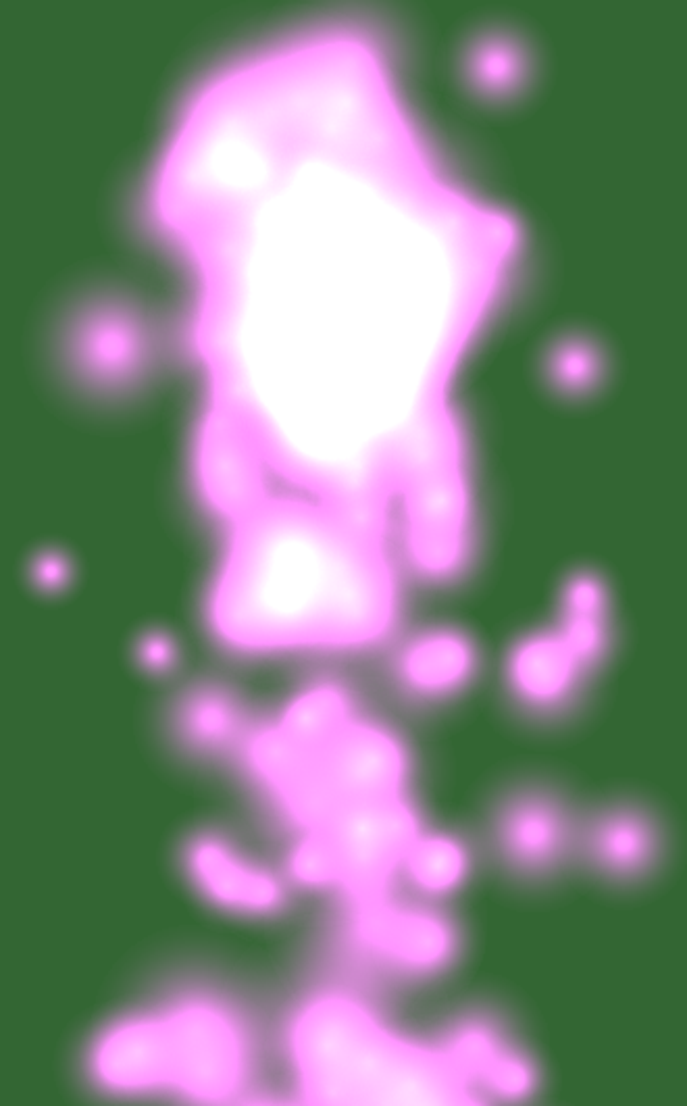
\includegraphics[scale=0.4]{bilder/ParticleFinal}
	\caption{Partikelsystem bei aktiviertem Blending und nicht-beschreibbarem Tiefenpuffer}
	\label{fig:ParticleFinal}
\end{figure}
%


\iffalse
\subsection{Billboarding}
\label{Kapitel_2_-_Unterkapitel_2.4}
%
Für ein besseres visuelles Ergebnis werden die Quads, auf die die Partikeltextur projiziert werden, immer orthogonal zur Blickrichtung der Kamera gerendert. Die Quads erfahren durch die
Modelview-Matrix keinerlei Rotationen. Um diesen Effekt, der als Billboarding bezeichnet wird, zu erreichen muss der Rotationsanteil der View-Matrix, also die linke obere 3x3-Matrix, auf die Einheitsmatrix gesetzt werden.

(Hier Abbildung ohne Billboarding)

Rotationsmatrizen sind Orthogonalmatrizen, das heißt, dass ihre Inversen ihren Transponierten entsprechen. Es genügt also beim Berechnen der Modelview-Matrix die obere linke 3x3-Matrix der Model-Matrix durch die Transponierte des Rotationsanteils der View-Matrix zu ersetzen. Da die Partikel in unserem System auch eine Größe haben wird die resultierende ModelView-Matrix noch mit einer Skalierungsmatrix multipliziert.
\fi